\chapter{Background}
\label{chap:background}
In this chapter some background on affective computing and BCI is provided. Then the circumplex model of affect is introduced together with the models for emotional correlates in the brain. Finally, the neuromarkers used as principal features for classification are presented.

\section{Affective Computing}
\label{sec:affective_computing}
All technologies that support the expression and the processing of human affective behaviours fall under the name of \ac{AC}, a relatively new branch of computer science named after Rosalind Picard’s work\cite{picard_mit_nodate}, that thoroughly described the practical methods and the ethical implications of building computers that can understand and express human emotions through the processing of behavioural, physiological, or conversational data. Building a very sophisticated \ac{AI} that mimics the human behaviour and can understand and replicate human emotions is still very far from the current state of art technology. Yet, the idea raises compelling questions on how we could interact with such entities and many the ethical implications. However, concrete applications able to perform Emotion-Recognition tasks are already on the market and in recent years have become a matter of great interest for researchers working in both academia and the industry. \ac{ER} is the task of recognizing human emotions by inferring them from different clues in the data. For example, from metadata collected from the usage of a software system; from data collected using wearable sensors such as accelerometers and gyroscopes; from photos and videos of facial expressions using computer vision; from text and voice samples processed using natural language processing techniques; from physiological measurements such as heart rate, dermal activity, and of course also brain activity.

The rapidly growing branch of \ac{AI}, mostly represented by machine learning algorithms, further fuels the development and the improvement of systems that can perform ER, by offering powerful techniques that can leverage the quantity of data to build fast and reliable systems more suitable for real-time tasks. Because of the nature of these data, it is possible to infer very sensitive behavioural and affective information from the users, exploitable by companies for commercial uses and marketing proposing, also evoking the unpleasant dreads of an Orwellian society where powerful corporations know exactly what people are thinking, feeling, desiring, or fearing and manipulate their emotions for “evil” purposes. Cases like the “Facebook emotional manipulation study” \cite{gertz_autonomy_2016} already demonstrate the interest and the ease for companies in inferring and manipulating their users’ emotions. Thus, philosophers and scholars already advocate for researchers and designers to design technology in a socially responsible behavior perspective 	\cite{tromp_design_2011}, so that users and companies are not tempted to misuse technology but rather use it to improve society. In the context of this research, a company building an intelligent system that can offer affective user experiences must ward the users’ control over their data and utilize these data with consensus and in respect of privacy laws, for example with anonymization of sensitive information. Even a music recommending system can raise serious ethical concerns: social functionalities might reveal sensitive information of a user to their network of friends, or groups of users might be targeted by affective promotional advertisement that has a negative impact on their emotional state.

In 2003, Picard also addressed with several criticisms the main challenges\cite{picard_affective_2003} faced by designers engaged in building machines with affective abilities. Some are relevant for the current study, in particular regarding the ability of sensing and recognizing emotions: Picard argued that the range of means, and modalities of emotion expression is very broad and hardly accessible, unlikely to be feasible in the near future. Another similar criticism regarded the accuracy of recognizing an individual’s emotional state from the available data and the difficulty in the articulation and assessment of one’s own feelings. While these criticisms still hold true, the technological developments of the last two decades of wearable sensing devices, including wearable \ac{BCIs}, greatly contributed to the collection of data that can be leveraged for affective computation, probably beyond Picard’s expectations. Brain activity, blood volume pressure, movement recorded through accelerometers, and heart rate have been used in several experiments for the \ac{ER} task and it has been proven possible by all these means, with different degrees of precision.The most relevant criticism probably regards the cognitive modeling of affective data. The progresses in psychological interpretation of idiosyncratic processes that characterize emotional responses are little and often supported by data collected in highly artificial lab environments. Multiple models for emotion assessments coexist in the emotion research community and there is still disagreement on what type of mechanisms mediate the effects of emotion. These models inevitably represent stylized stereotypes of emotional responsiveness and do not exactly correspond to the behavior and feelings in real people. While this study does not delve in evaluating the goodness of the emotional models, the use of a wearable device and the automated processing of data towards the realization of an online system are an attempt to simulate less artificial conditions. Further discussion about the subjective experiences of the participants (see Chapter \ref{chap:discussion}) gives further insights on the difficulties that arise in building affective systems from self-reported emotional responses.

\section{Wearable Brain-Computer Interfaces}
\label{sec:wearable_bci}
A \ac{BCI} often referred to as brain-machine interface, is a system that creates a pathway of direct communication between a brain and a computer. Research in \ac{BCI}  dates back to 1973 when Jacques Vidal named the field in his paper “Towards Brain-Computer communication”, and since then many technologies have been used to build this “bridge” between the human brain and machines; in their overview paper, Nicolas-Alonso and Gomez-Gil provide a good summary of the state-of-the-art \ac{BCIs} \cite{nicolas-alonso_brain_2012}. In short, a first categorization can be made between invasive or partially invasive \ac{BCIs}, implanted directly in the brain or on the skull, and non-invasive \ac{BCIs} that can be easily placed on the scalp. The main advantage of the first two categories resides in the greater amount and quality of data that is possible to collect. However, surgeries to implant electrodes can have negative outcomes for the subject including the formation of scar tissues, rejection of the electrodes or even worse infection. Consequently, invasive \ac{BCIs} are now mostly used in the experimental medical field where there is a necessity for a high temporal and spatial resolution to treat the patient's conditions. Non-invasive \ac{BCIs} instead often sacrifice spatial resolution and cannot effectively capture high frequencies in the brain signal due to the dispersion caused by the skull. In addition, they are affected by a higher presence of artefacts caused by environmental factors and muscular movements. Nevertheless, the easy and safe setup made non-invasive \ac{BCIs} the preferred choice for researchers and now the majority of published \ac{BCIs} work involves this type of \ac{BCIs}. The main technologies for non-invasive \ac{BCIs} are the following:
\begin{itemize}
\item \textbf{\ac{EEG}}: can record electrical brain activity from the scalp in the form of time series. Direct brain activity with good temporal resolution and bad spatial resolution.
\item \textbf{\ac{fMRI}}: can record brain activity by detecting changes in the blood flow. Structural brain activity with bad temporal resolution but good spatial resolution.
\item \textbf{\ac{fNIRS}}: can record brain activity based on neuro-vascular coupling. Indirect brain activity through oxygenation, bad temporal resolution, and good spatial resolution.
\item \textbf{ \ac{MEG}}: can record brain activity through the magnetic fields produced by the electrical currents in the brain. Direct brain activity with very good temporal resolution and spatial resolution is slightly better than EEG.
\end{itemize}
Among these technologies, \ac{EEG} has the best cost/capabilities compromise and eventually became the most popular for \ac{BCI}researchers to study\ac{EP} and \ac{ERPs}, thanks to the relatively cheap cost compared to \ac{MEG}, the good temporal resolution compared to \ac{fMRI} and \ac{fNIRS} and the good support provided by standardized software libraries for recording, streaming, and processing data like MNE\footnote{https://mne.tools} , EEGLab\footnote{https://sccn.ucsd.edu/eeglab/index.php} , OpenVibe\footnote{http://openvibe.inria.fr/}  and LabStreamingLayer\footnote{https://github.com/sccn/labstreaminglayer}. Except for some very rare cases, most of the portable \ac{BCIs} are based on \ac{EEG}.
\begin{figure}[h]
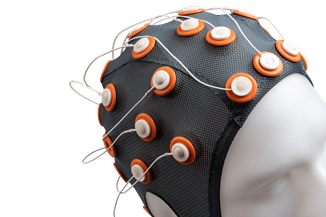
\includegraphics[width=10cm]{img/background/eeg_headcap.png}
\centering
\caption{An example of standard EEG headset}\label{fig_eeg_headcap}
\end{figure}
Standard EEG-based \ac{BCIs} usually require the subjects to wear a head-cap (Figure \ref{fig_eeg_headcap}) with 16, 32 or 64 electrodes placed over the scalp following the standard 10-20 system . These electrodes usually require the displacing of conductive gel to obtain a stable and qualitative signal. While this type of setup is acceptable for researchers in experimental environments, it is almost impossible to imagine a daily adoption from users. This problem is nowadays partly addressed by wearable EEG-capable headsets like Emotiv Epoc (Figure \ref{fig_emotiv}), Neurosky Mindwave, Muse Headband, NextMind, Melomind (Fig. 4) and many others, that mostly feature EEG capabilities with 2 up to 16 soft dry electrodes, and do not require conductive gel to capture the electric signal of the brain. While the quality of the signal is not usually as good and complete as the standard EEG-based devices, the setup of these portable \ac{BCIs} is seamless and often requires just a simple calibration making them suitable for both researchers and consumers.
\begin{figure}[h]
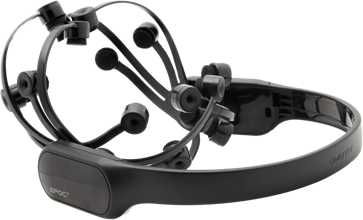
\includegraphics[width=10cm]{img/background/fig_emotiv.png}
\centering
\caption{Emotiv Epoc+ portable EEG device with 14 electrodes}\label{fig_emotiv}
\end{figure}
The experimental and analytical phases of this study have been conducted in collaboration with myBrainTechnologies, a startup based in Paris that designed Melomind to offer a real-time auditory neurofeedback application to induce a relaxation state. Apart from its designed purpose, Melomind is a fully featured \ac{BCI} that comes in two versions, standard and Q+. The standard version used in the experiment features Bluetooth headphones with 2 textile reference electrodes and 2 dry electrodes for recording that can be placed on the parietal area in correspondence of the P3/P4 electrodes or in the frontal area in correspondence of the AF3/AF4 electrodes on the 10-20 system. 
